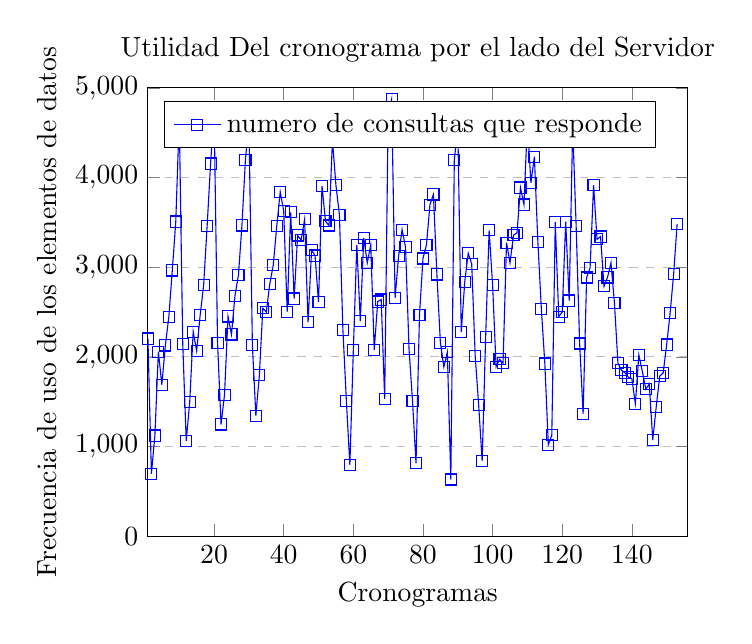
\begin{tikzpicture}
\begin{axis}[
    title={Utilidad Del cronograma por el lado del Servidor},
    xlabel={Cronogramas},
    ylabel={Frecuencia de uso de los elementos de datos},
    xmin=1, xmax=156,
    ymin=0, ymax=5000,
    xtick={},
    ytick={},
    legend pos=north west,
    ymajorgrids=true,
    grid style=dashed,
]

\addplot[
    color=blue,
    mark=square,
    ]
    coordinates {
%UTILIDAD TOTAL
%(cronograma, numero cues que usan al cronograma)
(1,2204)
(2,696)
(3,1122)
(4,2058)
(5,1689)
(6,2127)
(7,2444)
(8,2964)
(9,3509)
(10,4663)
(11,2144)
(12,1063)
(13,1494)
(14,2281)
(15,2066)
(16,2463)
(17,2799)
(18,3457)
(19,4156)
(20,4750)
(21,2156)
(22,1246)
(23,1577)
(24,2451)
(25,2250)
(26,2683)
(27,2912)
(28,3466)
(29,4195)
(30,4633)
(31,2133)
(32,1343)
(33,1794)
(34,2543)
(35,2501)
(36,2814)
(37,3022)
(38,3457)
(39,3840)
(40,3626)
(41,2504)
(42,3611)
(43,2650)
(44,3354)
(45,3302)
(46,3533)
(47,2385)
(48,3190)
(49,3130)
(50,2610)
(51,3907)
(52,3513)
(53,3465)
(54,4415)
(55,3914)
(56,3585)
(57,2303)
(58,1511)
(59,794)
(60,2077)
(61,3247)
(62,2399)
(63,3327)
(64,3048)
(65,3251)
(66,2076)
(67,2617)
(68,2639)
(69,1531)
(70,4702)
(71,4875)
(72,2657)
(73,3127)
(74,3419)
(75,3222)
(76,2085)
(77,1505)
(78,813)
(79,2470)
(80,3097)
(81,3250)
(82,3696)
(83,3811)
(84,2919)
(85,2159)
(86,1888)
(87,2051)
(88,632)
(89,4193)
(90,4570)
(91,2277)
(92,2838)
(93,3156)
(94,3036)
(95,2011)
(96,1462)
(97,839)
(98,2219)
(99,3411)
(100,2803)
(101,1891)
(102,1973)
(103,1929)
(104,3274)
(105,3049)
(106,3357)
(107,3382)
(108,3888)
(109,3699)
(110,4615)
(111,3940)
(112,4232)
(113,3285)
(114,2536)
(115,1925)
(116,1020)
(117,1124)
(118,3502)
(119,2449)
(120,2500)
(121,3507)
(122,2628)
(123,4561)
(124,3456)
(125,2149)
(126,1365)
(127,2885)
(128,2991)
(129,3914)
(130,3310)
(131,3342)
(132,2786)
(133,2886)
(134,3048)
(135,2597)
(136,1930)
(137,1851)
(138,1823)
(139,1772)
(140,1757)
(141,1477)
(142,2021)
(143,1840)
(144,1640)
(145,1697)
(146,1073)
(147,1443)
(148,1784)
(149,1822)
(150,2137)
(151,2492)
(152,2924)
(153,3482)
    };
    \legend{numero de consultas que responde}

\end{axis}
\end{tikzpicture}

